\documentclass[12pt, a4paper]{scrartcl}

\usepackage[utf8]{inputenc}
\usepackage[ngerman]{babel}
\usepackage{float}
\usepackage{listings}
\usepackage{color}
\usepackage{xcolor}
\usepackage{graphicx}
\usepackage{caption}
\usepackage{subcaption}
\usepackage{algorithm2e}
\usepackage{amsmath}
\usepackage{amsfonts}
\usepackage{mathtools}
\usepackage[a4paper,%
top=10mm, bottom=10mm, left=10mm, right=15mm]{geometry}
% \usepackage{isodate}

\graphicspath{{./images/}}

%%%%%%%%%%%%%%%%%%%%%%%%%%%%%% Newcommands
\newcommand{\bigO}{\mathcal{O}}
\renewcommand{\implies}{\Rightarrow}
\newcommand{\lif}{\Leftarrow}
\newcommand{\liff}{\Leftrightarrow}
\newcommand{\abs}[1]{|#1|}
\newcommand{\imgwidth}{.7\textwidth}

\DeclarePairedDelimiter{\floor}{\lfloor}{\rfloor}
\DeclarePairedDelimiter{\ceil}{\lceil}{\rceil}

%%%%%%%%%%%%%%%%%%%%%%%%%%%%%% Listings
\newfloat{listing}{thp}{lop}
\floatname{listing}{Code snippet}

 \lstset{
         basicstyle=\footnotesize\ttfamily, % Standardschrift
         numbers=left,               % Ort der Zeilennummern
         numberstyle=\tiny,          % Stil der Zeilennummern
         %stepnumber=2,               % Abstand zwischen den Zeilennummern
         numbersep=3pt,              % Abstand der Nummern zum Text
         %tabsize=2,                  % Groesse von Tabs
         extendedchars=true,         %
         breaklines=true,            % Zeilen werden Umgebrochen
         keywordstyle=\color{blue},
         frame=tb,
%         keywordstyle=[1]\textbf,    % Stil der Keywords
%         keywordstyle=[2]\textbf,    %
%         keywordstyle=[3]\textbf,    %
%         keywordstyle=[4]\textbf,   \sqrt{\sqrt{}} %
         stringstyle=\color{white}\ttfamily, % Farbe der String
 %        showspaces=false,           % Leerzeichen anzeigen ?
         showtabs=false,             % Tabs anzeigen ?
         % xleftmargin=17pt,
%         framexleftmargin=17pt,
%         framexrightmargin=5pt,
%         framexbottommargin=4pt,
         backgroundcolor=\color{lightgray},
%         showstringspaces=false      % Leerzeichen in Strings anzeigen ?        
 }

\author{Michael Floßmann}

\begin{document}
\tableofcontents{}
\section{Sorting}
\label{sec:sorting}
Problem:
\begin{itemize}
\item $n$ elements $\mathbf{x}=(x_1,x_2,...,x_n)$
\item Output: $\mathbf{x^*}$ ordered s.t. $x^*_i\le x^*_{i+1}$
\end{itemize}

\subsection{MinSort}
\label{sec:minsort}
\begin{table}[!h]
  \centering
  \begin{tabular}{lc}
    Complexity:&$\mathcal{O}(n^2)$
  \end{tabular}
  \caption{Minsort attributes}
  \label{tab:minsort}
\end{table}
\begin{enumerate}
\item Find the minimum and switch the value with the \emph{first} position.
\item Find the minimum and switch the value with the \emph{second} position.
\item ...
\end{enumerate}
\begin{listing}
  \lstinputlisting[language=Python, inputencoding=latin1]{minsort.py}
  \caption{minsort()}
\end{listing}
\subsection{Heapsort}
\label{sec:minsort}
% \begin{table}[!h]
%   \centering
%   \begin{tabular}{lc}
%     Complexity:&$\mathcal{O}(n^2)$
%   \end{tabular}
%   \caption{Minsort attributes}
%   \label{tab:minsort}
% \end{table}
\subsubsection{Binary heap:}
\begin{itemize}
\item Binary tree (preferably complete)
\item \textbf{Heap property:} Each child is smaller(/larger) than the parent element.
\end{itemize}
\begin{figure}[!htbp]
  \centering
  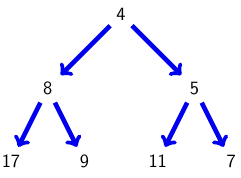
\includegraphics{minheap}
  \caption{Valid min heap}
  \label{fig:minheap}
\end{figure}
Children of node $i$: $2i+1$ and $2i+2$\\
Parent of node $i$: $\mathrm{floor}(\frac{i-1}{2})$

 \subsubsection{Algorithm}
 \label{sec:heapsort_algorithm}
 \textbf{Sifting down:} Check whether current node violates the heap condition. If so: Switch with smaller child and repeat step with the new child until you reach the bottom.\\
 \textbf{Heapsort():}
 \begin{enumerate}
 \item Heapify list by sifting down from the bottom up.
 \item While elements are in the heap
   \begin{enumerate}
   \item Remove root element and add it to the sorted list.
   \item Put the last element in the heap to the root position.
   \item Sift down from the root position
   \end{enumerate}
 \end{enumerate}

 \subsubsection{Attributes}
\label{sec:heapsort_attr}
\begin{itemize}
\item First: \emph{heapify} array of $n$ elements
  \begin{itemize}
  \item Depends on depth of tree
  \item In general: costs are linear with path length and number of nodes.
  \end{itemize}
\item Then: until all $n$ elements are sorted:
  \begin{itemize}
  \item constant stuff
  \item sifting
  \end{itemize}
\end{itemize}
\fbox{\textbf{Total runtime:} $T(n)\le 6 \cdot n \log_2n \cdot C$}

% \begin{algorithm}[H]
%   \KwData{unsorted list $\mathbf{x}$ of size $n$}
%   \KwResult{sorted list $\mathbf{x}^*$}
%   \SetKwFunction{sort}{sort}
%   \SetKwFunction{siftdown}{siftdown}
%   \SetKwProg{func}{Function}{}{}
%   \func{\sort{list}}{
%   \While{elements in heap}
%     remove smallest element\;
%     put last node into the root spot\;
%     \siftdown{heap}\;}
%    \KwRet\;}{}
%   \func{\siftdown{heap}}{
%     fixed = False\;
%     $i$ = root.index\;
%     \While{fixed == false}{
%       \If{node.value $>\mathrm{child_1.value}$}{
%       switch $\mathrm{child}_1$ and \emph{node}\;
%       $i$ = $\mathrm{child_1.index}$\;}
%     \ElseIf{node.value $>\mathrm{child_2.value}$}{
%       switch $\mathrm{child}_2$ and \emph{node}\;
%       $i$ = $\mathrm{child_2.index}$\;}
%     \Else{fixed = True}}
%   }
  
%   \nl \KwRet\;}
%   \caption{Algorithm with procedure}
% \end{algorithm}
 
\section{Runtime}
\label{sec:runtime}
Runtime is dependent on (other than efficiency of code):
\begin{itemize}
\item Specs of the computer
\item Applications in the background
\item Compiler effiency
\end{itemize}

\subsection{$\mathcal{O}-Notation$}
\label{sec:O-notation}
\[f\in\mathcal{O}(g)\Rightarrow f(n)\le C\cdot g(n)\forall\]\\
Formal:
\begin{equation}
\mathcal{O}(g)=\{f:\mathbb{N}\rightarrow\mathbb{R}|\exists n_0\in\mathbb{N}, \exists C>0, \forall n>n_0:f(n)\le C\cdot g(n)\}
\end{equation}
\begin{figure}[htbp]
  \centering
  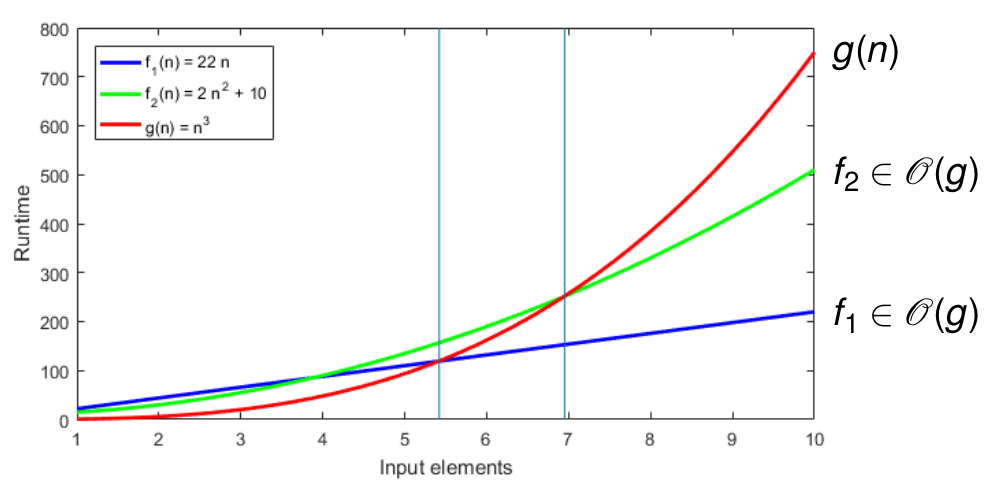
\includegraphics[width=.9\textwidth]{bigO}
  \caption{Illustration of $\mathcal{O}$}
  \label{fig:big-O-illustration}
\end{figure}
\begin{itemize}
\item We are only interested in the term with the highest order (i.e. the fastest growing summand), others are ignored.
\item $f(n)$ is limited \emph{from above} by $C\cdot g(n)$
\end{itemize}

\subsection{$\Omega$-Notation}
\label{sec:omega-notation}
$f\in\Omega(g)\Rightarrow f$ is growing at least as fast as $g$.
\[f\in\mathcal{O}(g)\Rightarrow f(n)\ge C\cdot g(n)\forall\]\\
Formal:
\[\Theta(g)=\{f:\mathbb{N}\rightarrow\mathbb{R}|\exists n_0\in\mathbb{N}, \exists C>0, \forall n>n_0:f(n)\ge C\cdot g(n)\}
\]
\begin{itemize}
\item We are only interested in the term with the highest order (i.e. the fastest growing summand), others are ignored.
\item $f(n)$ is limited \emph{from below} by $C\cdot g(n)$
\end{itemize}
\subsection{$\Theta$-Notation}
\label{sec:Theta-notation}
$f\in\Theta(g)\Rightarrow f$ is growing at the same rate as $g$.
\[f\in\mathcal{O}(g)\Rightarrow f(n)\ge C\cdot g(n)\forall\]\\
Formal:
\[\Theta(g)=\mathcal{O}(g)\cap\Omega(g)
\]

\subsection{Summary}
\label{sec:O-notation}
\begin{itemize}
\item With $\bigO$ notation we're interested in $n\rightarrow\infty$. 
\item $\bigO$ only applies for $n\ge n_0$.
\item \textbf{Attention:} $n_0$ does \textbf{not} have to be a small number.
\end{itemize}


\subsubsection{Limits}
\begin{align}
  f\in\mathcal{O}(g)&\Leftrightarrow\lim_{N\rightarrow\infty}\frac{f(n)}{g(n)}<\infty\\
  f\in\Omega(g)&\Leftrightarrow\lim_{N\rightarrow\infty}\frac{f(n)}{g(n)}>0\\
  f\in\Theta(g)&\Leftrightarrow0<\lim_{N\rightarrow\infty}\frac{f(n)}{g(n)}<\infty\\
\end{align}

\subsubsection{Algebraic rules}
\paragraph{Transivity}
\begin{align}
  f\in\mathcal{O}(g)\land g\in\mathcal{O}(h)&\Rightarrow f \in \mathcal{O}(h)\\
  f\in\Omega(g)\land g\in\Omega(h)&\Rightarrow f \in \Omega(h)\\
  f\in\Theta(g)\land g\in\Theta(h)&\Rightarrow f \in \Theta(h)\\
\end{align}

\paragraph{Symmetry}
\begin{align}
  f\in\mathcal{O}(g)&\Leftrightarrow g \in \Omega(f)\\
  f\in\Theta(g) &\Leftrightarrow g\in\Theta(f)
\end{align}

\paragraph{Reflexivity}

\begin{equation}
  f\in\Theta(f), f\in\Omega(f), f\in\mathcal{O}(f)
\end{equation}
\paragraph{Trivial}
  \begin{align}
    f&\in\bigO(f)\\
    k\cdot\bigO(f) &= \bigO(f)\\
    \bigO(f+k) &= \bigO(f)
  \end{align}
\paragraph{Addition}
  \begin{equation}
    \bigO(f)+\bigO(g)=\bigO(\max\{f,g\})
  \end{equation}
\paragraph{Multiplication}
  \begin{equation}
    \bigO(f)\cdot\bigO(g)=\bigO(f\cdot g)
  \end{equation}
\begin{figure}[!htbp]
  \centering
  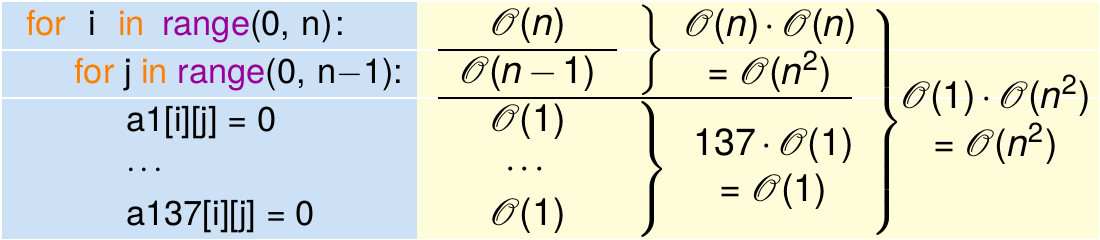
\includegraphics[width=.8\textwidth]{bigO_loops}
  \caption{Behavior of $\bigO$ in loops}
  \label{fig:bigO_loops}
\end{figure}
\begin{figure}[!htbp]
  \centering
  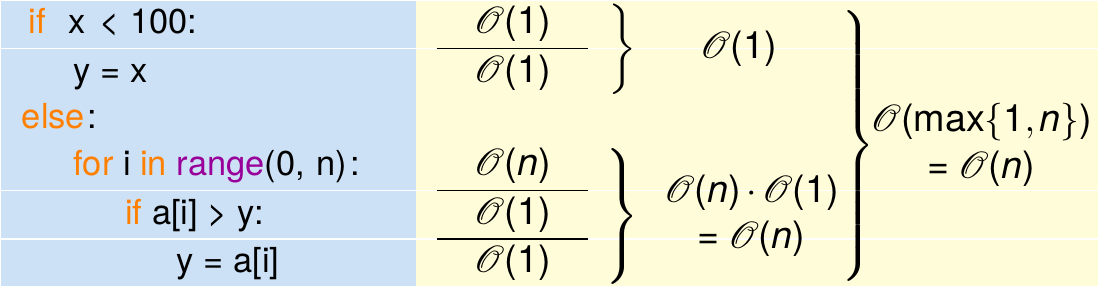
\includegraphics[width=.8\textwidth]{bigO_conditions}
  \caption{Behavior of $\bigO$ in conditions}
  \label{fig:bigO_conditions}
\end{figure}
\begin{table}[!htbp]
  \centering
  \caption{Common runtime types}
  \label{tab:common_runtime}
  \begin{tabular}{c|l}
    Runtime&Growth in time\\\hline\hline
    $f\in\Theta(1)$&Constant\\
    $f\in\Theta(\log_k n)$&Logarithmic\\
    $f\in\Theta(n)$&Linear\\
    $f\in\Theta(n\log n)$&n-log-n time (almost linear)\\\hline
    $f\in\Theta(n^2)$&Squared time\\
    $f\in\Theta(n^3)$&Cubic time\\
    $f\in\Theta(n^k)$&Polynomial time\\\hline
    $f\in\Theta(k^n),\ f\in\Theta(2^n)$&Exponential Time\\
  \end{tabular}
\end{table}

\newpage{}
\section{Associative array}
\label{sec:associative_array}

\textbf{Associative arrays} are arrays in which you access the elements not via index, but via a \emph{key}.
\begin{center}
  A[``Mueller'']=``0140-373830''
\end{center}
\textbf{Disadvantage:} Lookup takes long ($\Theta(n)$)

\section{Hashmap}
\label{sec:hashmap}
Idea: Mapping the keys onto indices with a \emph{hash function} $h$ and store the data in a regular array.
\begin{itemize}
\item \textbf{Advantage:} Lookup takes $\Theta(1)$ (in the best case).
\item \textbf{Problem:} If $h(x_i)=h(x_j), x_i\ne x_j\Rightarrow$ a \emph{Collision} occurs. (Quite common, see the Birthday problem)
\end{itemize}

\subsection{Buckets}
\label{sec:hashmap_buckets}
Simple solution to collision: Lists (buckets) as entries to hashmaps
\begin{itemize}
\item Best case: $n$ keys equally distributed over $m$ buckets $\Rightarrow \approx \frac{m}{n}$
\item Worst case: All $n$ keys mapped onto the same bucket (\emph{degenerated hash table}) $\Rightarrow$ Searching runtime $\Theta(n)$
\end{itemize}

\subsection{Universal hashing}
\label{sec:universal_hashing}
\begin{itemize}
\item Way of avoiding degenerated hash tables
\item Define a set of hash functions.
\item Choose a random hash function so that the expected result is an equal distribution over the buckets.
\item Since a big universe is mapped onto a small set, no hash function is good/suitable for all key sets
\end{itemize}

\paragraph{Definition}
\begin{itemize}
\item $\mathbb{U}$: Universe of possible keys
\item $\mathbb{S}\subseteq\mathbb{U}$: Set of used keys
\item $m$: Size of the hash table $T$
\item $\mathbb{H}=\{h_1,h_2,...,h_n\}:$ Set of hash functions with $h_i:\mathbb{U}\rightarrow\{0,...,m-1\}$
\item[$\Rightarrow$] $\frac{|\mathbb{S}|}{m}:=$ \emph{table load}
\item Runtime should be $\bigO(1+\frac{|\mathbb{S}|}{m})$
\end{itemize}
$\mathbb{H}$ is \emph{$c$-universal} $\Leftarrow \forall x,y\in\mathbb{U}|x\ne y:$
\begin{equation*}
  \overbrace{\frac{|h\in\mathbb{H}:h(x)=h(y)|}{\underbrace{|\mathbb{H}|}_{\mathrm{No.\ of\ hash\ functions}}}}^{\mathrm{No.\ of\ hash\ functions\ that\ create\ collisions}}
  \le c\cdot\frac{1}{m},\quad c\in \mathbb{R}
\end{equation*}
Which means:
\begin{equation*}
  p\underbrace{(h(x)=h(y))}_\mathrm{Collision}\le c\cdot \frac{1}{m}
\end{equation*}
\begin{figure}[!htbp]
  \centering
  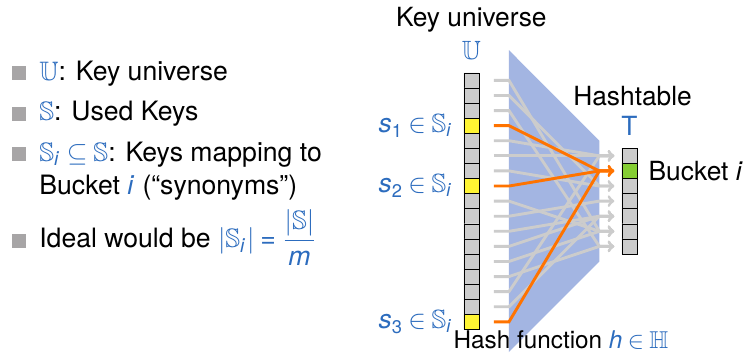
\includegraphics[width=.9\textwidth]{universal_hashing}
  \caption{Schematic for universal hashing}
  \label{fig:universal_hashing}
\end{figure}

\paragraph{Lookup time}
\begin{itemize}
\item $\mathbb{H}$: $c$-universal class of hash functions
\item $\mathbb{S}$: set of keys
\item $h\in\mathbb{H}$: randomly selected hash functions
\item $\mathbb{S}_i$:= the key $x$ for which $h(x)=i$
\end{itemize}
Then, the average bucketsize is:
\begin{equation}
  \mathbb{E}\{|\mathbb{S}_i|\}\le 1+c\cdot\frac{|\mathbb{S}|}{m}
\end{equation}
Particularly:
\begin{equation}
  m=\Omega(|\mathbb{S}|)\Rightarrow\mathbb{E}\{|\mathbb{S}_i|\}=\bigO(n)
\end{equation}

\paragraph{Proof}\mbox{}\\
\textbf{Given:}
\begin{itemize}
\item Pick two random keys $x,y\in\mathbb{S}|x\ne y$ and a random, $c$-universal hash function $h\in\mathbb{H}$
\item Probability of a collision:
  \[P(h(x)=h(y))\le \frac{c}{m}\]
\end{itemize}
\textbf{To proof:}
\[\mathbb{E}\{|\mathbb{S}_i|\}\le 1 + c\cdot\frac{|\mathbb{S}|}{m}\]
\textbf{Proof:}
\[\mathbb{S}_i=\{x\in\mathbb{S}:h(x)=i\}\]
if $\mathbb{S}_i=\emptyset\implies\abs{\mathbb{S}_i}=0$; otherwise, let $x\in\mathbb{S}_i$ be any key:
\begin{align*}
I_y&:=\left\{
  \begin{array}{l}
    1,\quad \mathrm{if\ } h(y)=i\\
    0,\quad \mathrm{else}
  \end{array}\right.
  y\in\mathbb{S}\backslash \{x\}\\
  \implies \abs{\mathbb{S}_i}&=1+\sum_{y\in\mathbb{S}\backslash x}I_y\\
  \implies \mathbb{E}\{\abs{\mathbb{S}_i}\}&=\mathbb{E}
  \left\{
  1+\sum_{y\in\mathbb{S}\backslash x}I_y
  \right\} = 1 + \sum_{y\in\mathbb{S}\backslash x} \underbrace{\mathbb{E}\{I_y\}}_{\le c\cdot\frac{1}{m}}
\end{align*}
\begin{align*}
  \implies 1 + \sum_{y\in\mathbb{S}\backslash x}\mathbb{E}\{I_y\}&\le 1+ \sum_{y\in\mathbb{S}\backslash x} c\cdot\frac{1}{m}\\
                                                                 &=1+(\abs{\mathbb{S}}-1)\cdot c\cdot\frac{1}{m}\\
                                                                 &\le 1+ c\cdot\frac{\abs{\mathbb{S}}}{m}\\
  \mathbb{E}\{\abs{\mathbb{S}_i}\}&=1+\sum_{y\in\mathbb{S}\backslash x}\mathbb{E}\{I_y\}
                                    \le 1+c\cdot\frac{\abs{\mathbb{S}}}{m}\quad \mathrm{q.e.d.}
\end{align*}

\paragraph{Examples for universal hashing}
\begin{itemize}
\item $p$: big prime number, $p>m$, and $p\ge\abs{\mathbb{U}}$
\item $\mathbb{H}$: Set of all $h$ for which:
  \[h_{a,b}(x)=((a\cdot x+b)\mod p) \mod m\]
  where $1\le a < p,\quad 0\le b < p$
\item This is $\approx 1$-universal %TODO: Maybe include proof?
\end{itemize}

\subsection{Rehashing}
\label{sec:rehashing}
\begin{itemize}
\item \emph{Rehash}: New hash table with new random hash function
  \begin{itemize}
  \item[$\rightarrow$] Expensive, but rarely done $\implies$ average cost is low
  \end{itemize}
\end{itemize}

\subsection{Linked lists for buckets}
\label{sec:linked_lists_buckets}
\begin{itemize}
\item Each bucket is a linked list.
\item If a collision occurs the new keys are sorted into, or appended at the end of the list.
\item Best case: Operations take $\bigO(1)$
\item Worst case: $\bigO(n)$ e.g. for degenerated tables
\end{itemize}

\subsection{Open Addressing}
\label{sec:open_addressing}
\begin{itemize}
\item For colliding keys we choose a new free entry.
\item A \emph{probe sequence} determines in which sequence the hash table is searched for a free bucket.
  \begin{itemize}
  \item Entries are iteravly checked, until a free one is found where the element can be inserted.
  \item If a lookup doesn't find the corresponding entry, probing has to be performed, until the element or a free entry is found.
  \end{itemize}
\end{itemize}

\paragraph{Definitions}
\begin{itemize}
\item $h(s)$: Hash function for key $s$
\item $g(s,j)$: Probing function for key $s$ with overflow positions $j\in\{0,...,m-1\}$,\\ e.g. $g(s,j)=j$
\item The \emph{probe sequence} is calculated by:
  \begin{equation}
    \label{eq:probe_sequence}
    h(s,j)=(h(s)-g(s,j))\quad \mod m\in\{0,...,m-1\}
  \end{equation}
  \begin{figure}[!htbp]
    \centering
    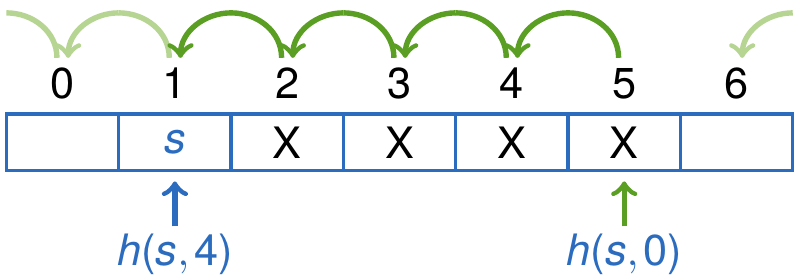
\includegraphics[width=0.7\textwidth]{probe_sequence}
    \caption{Linear sequence ($g(s,j)=j$)}
    \label{fig:probe_sequence}
  \end{figure}
\end{itemize}

\paragraph{Linear probing $g(s,j)=j$}

\begin{itemize}
\item $g(s,j)$ clips from $0$ to $m-1$.
\item Can result in primary clustering 
\item[$\implies$] Hash collisions result in higher probability of hash collisions in close entries (hence, $\bigO(n)$ for lookup)
\end{itemize}

\paragraph{Squared probing}
\begin{itemize}
\item Motivation: Avoid local clustering
  \begin{equation}
    g(s,j):=(-1)^j\floor{\frac{j}{2}}^2
  \end{equation}
\item Resulting probe sequence:
  \[h(s),h(s)+1, h(s)-1, h(s)+4, h(s)-4,...\]
\begin{figure}[!htbp]
  \centering
  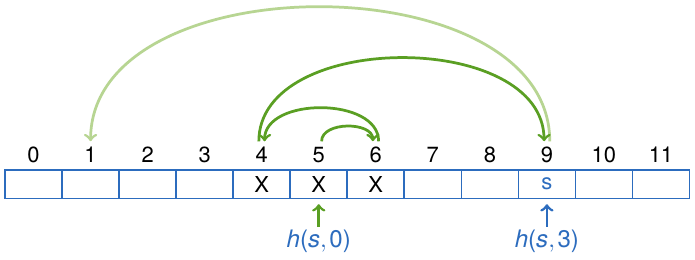
\includegraphics[width=.7\textwidth]{squared_probing}
  \caption{Squared probe sequence}
  \label{fig:squared_probing}
\end{figure}
\item If $m$ is a prime number s.t. $m=4\cdot k+3$, then the probe sequence is a permutation of the indices of the hash tabels
\item Problem: Secondary clustering
\end{itemize}
\paragraph{Uniform probing}

\begin{itemize}
\item So far: $g(s,j)$ independent of $s$
\item \emph{Uniform probing}: $g(s,j)$ also dependent on the key $s$
\item Advantage: Prevents clustering, because different keys with the same hash value produce a different probe sequence
\item Disadvantage: Hard to implement
\end{itemize}
\paragraph{Double hashing}

\begin{itemize}
\item Use two independent hash functions $h_1(s), h_2(s)$
  \begin{equation}
    h(s,j)=(h_1(s)+j\cdot h_s(s))\mod m
  \end{equation}
\item Works well in practical use
\item Approximation of uniform probing
\item \textbf{Double hashing by} \textsc{Brent}
  \begin{itemize}
  \item Test if $h(s_1,1)$ is free
  \item If yes, move $s_1$ from $h(s_1,0)$ to $h(s_1,1)$ and insert $s_2$ at $h(s_2,0)$
  \end{itemize}

\end{itemize}

\paragraph{Ordered hashing}
\begin{itemize}
\item If a collission occurs for the keys $s_0$ and $s_1$, insert the smaller key and search a new position for the bigger according to the probe sequence.
\item[$\implies$] Unsuccessful search can be aborted sooner
\end{itemize}

\paragraph{Robin-Hood Hashing}
\begin{itemize}
\item If two keys $s_1, s_2$ collide, compare the length of the sequence $j_1$ and $j_2$.
\item The key with the bigger search sequence is inserted at $p_1$, the other one gets reassigned according to the sequence.
\end{itemize}

\paragraph{Insert and Remove}
\begin{itemize}
\item \textbf{Problem}:
  \begin{enumerate}
  \item Key $s_1$ is inserted at $p_1$
  \item Key $s_2$ collides with $s_2$ at $p_1$ $\leftarrow$ gets inserted at $p_2$, due to probing order
  \item $s_1$ removed $\implies$ $s_2$ is virtually lost
  \end{enumerate}
\item \textbf{Solution:}
  \begin{itemize}
  \item Remove: Elements are marked as removed, but not deleted.
  \item Insert: Elements marked as removed are overwritten.
  \end{itemize}
\end{itemize}

\section{Priority Queue}
\label{sec:priority_queue}
\begin{itemize}
\item Stores a set of elements
\item Each element contains a key and a value.
\item There is a total order (e.g. $\le$) defined on the keys (heap).
\item Operations
  \begin{itemize}
  \item \texttt{insert(key, value)}:
    \begin{enumerate}
    \item Append element at the end of the array
    \item Repair heap condition
    \end{enumerate}
  \item \texttt{getMin()}: Return the first element or \texttt{None} if heap empty.
  \item \texttt{deleteMin()}:
    \begin{enumerate}
    \item Delete root of heap.
    \item Put last element at the root.
    \item Repair heap condition. (only up/down)
    \end{enumerate}
  \end{itemize}
\item Additional operations:
  \begin{itemize}
  \item \texttt{changeKey(item, key)}:
    \begin{enumerate}
    \item Change key value.
    \item Repair heap condition. (only up/down)
    \end{enumerate}

  \item \texttt{remove(item)}:
    \begin{enumerate}
    \item Replace element with the last element and shrink heap by one.
    \item Repair heap condition. (only up/down)
    \end{enumerate}
    \begin{figure}[htbp]
      \centering
      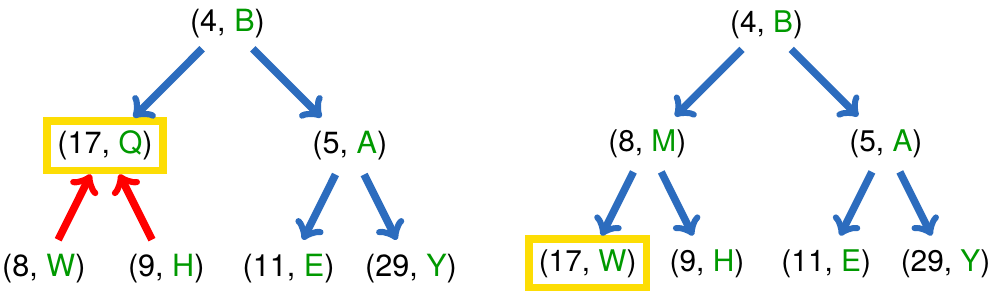
\includegraphics[width=0.7\textwidth]{sift_up}
      \caption{Sift up}
      \label{fig:sift_up}
    \end{figure}
    \begin{figure}[htbp]
      \centering
      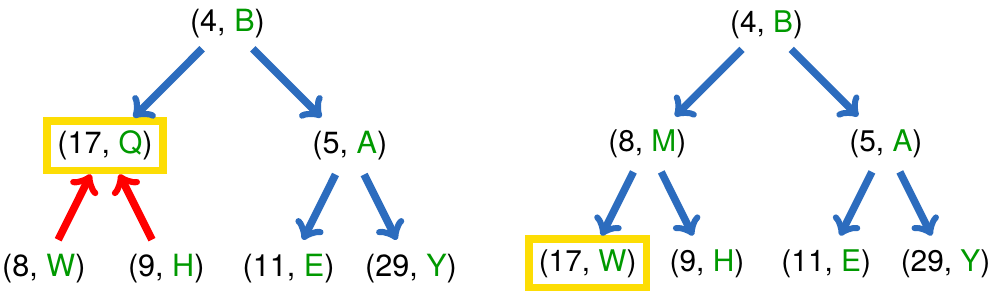
\includegraphics[width=0.7\textwidth]{sift_up}
      \caption{Sift down}
      \label{fig:sift_down}
    \end{figure}
  \end{itemize}
\item Multiple elements with the same key are allowed.
\item \textbf{Each element has to store its' current position in the heap.}
\end{itemize}

\section{Static and dynamic arrays}
Static arrays have a fixed size (has to be known at compile time).

\subsection{Dynamic arrays}
\label{sec:dynamic_arrays}
Resizing an array:
\begin{enumerate}
\item Allocate array with new size
\item Copy entries from old array to new array
\end{enumerate}

\paragraph{Naive implementation}
\begin{itemize}
\item Resize array before each append to the exact needed size
\item Runtime: $\bigO(n^2)$
\end{itemize}

\paragraph{Constantly generous allocation}
\begin{itemize}
\item Allocate more space than needed.
\item Amount of over-allocation $C$ is constant.
\item Runtime: still $\bigO(n^2)$
\begin{figure}[htbp]
  \centering
  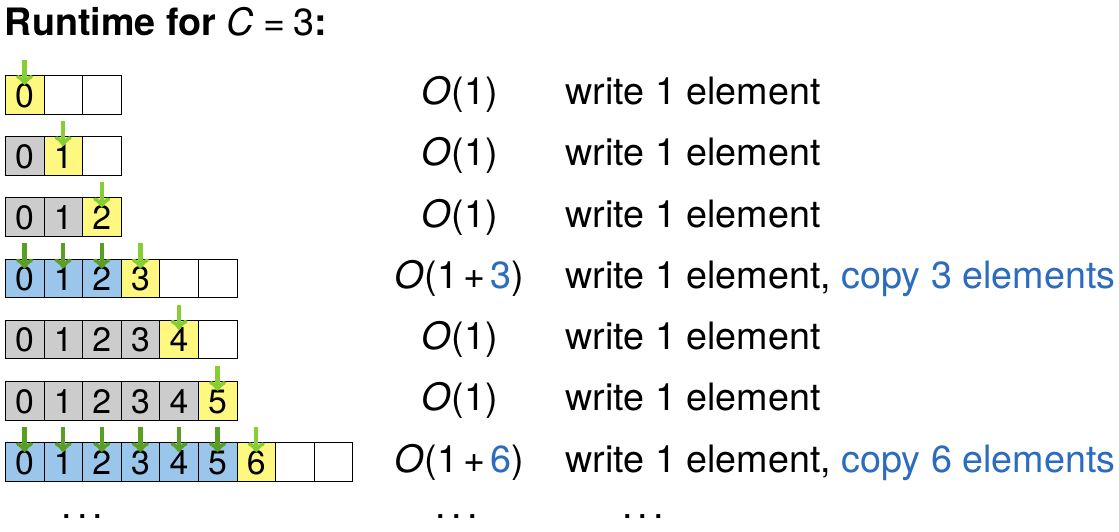
\includegraphics[width=.7\textwidth]{constant_reallocation}
  \caption{Runtime of constantly generous reallocation}
  \label{fig:constant_reallocation}
\end{figure}
\item Most of the append operations now cost $\bigO(1)$, every $C$ steps, cost of copying are added.\\$\implies$ We're getting faster
\end{itemize}

\paragraph{Variable overallocation}
\begin{itemize}
\item Idea: Double size of the array for reallocation
\item Runtime:
  \begin{itemize}
  \item Now, all appends cost $\bigO(1)$
  \item Every $2^i$ steps we have to add the cost $A\cdot2^i$ ($i=0,1,2,...,k; k=\floor{\log_2(n-1)}$)
    \begin{align*}
      T(n)&=n\cdot A+ A\cdot\sum^k_{i=0}2^i=n\cdot A+A(2^{k+1}-1)\\
          &\le n\cdot A+ A\cdot 2^{k+1}\\
          &=n\cdot A + 2\cdot A\cdot 2^k\\
          &\le n\cdot A + 2\cdot A\cdot n\\
          &=3A\cdot n\\
          &\in\bigO(n)
    \end{align*}
  \end{itemize}
\item Further improvement:
  \begin{itemize}
  \item Shrink array by half, if it is half-full.
  \item Only shrink it to 75\% to optimize appending afterwards.
  \end{itemize}
\end{itemize}

\subsection{Amortized analysis}
\label{sec:amortized_analysis}
\begin{itemize}
\item $n$ instructions $O=\{O_1,...,O_n\}$
\item $s_i$: Size after operation $i$, $s_0:=0$
\item $c_i$: Capacity after operation $i$, $c_0:=0$
\item $T(O_i)$: Cost of operation $i$:
  \begin{align*}
    \mathrm{Reallocation{:}\ }&T(O_i)\le A\cdot s_i\\
    \mathrm{Insert/Delete{:}\ }&T(O_i)\le A
  \end{align*}
  \begin{figure}[htbp]
    \centering
    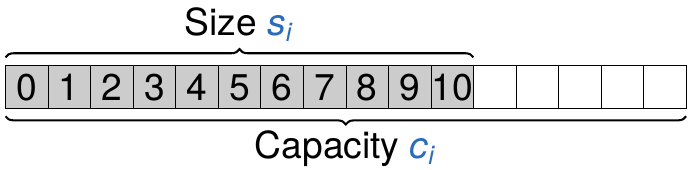
\includegraphics[width=0.7\textwidth]{static_array_capacity}
    \caption{Static array with capacity $c_i$}
    \label{fig:static_array_capacity}
  \end{figure}
\item Implementation:
  \begin{itemize}
  \item If $O_i=$ append and $s_{i-1}=c_{i-1}$:
    \begin{itemize}
    \item Resize array to $c_i=\floor{\frac{3}{2}s_i}$
    \item $T(O_i)=A\cdot s_i$
    \end{itemize}
    \begin{figure}[htbp]
      \centering
      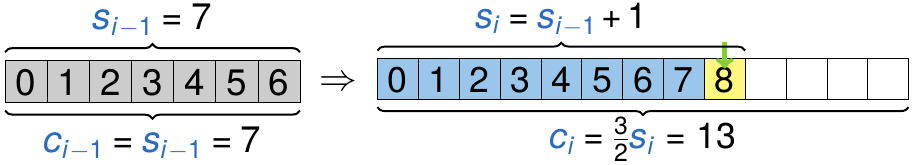
\includegraphics[width=\imgwidth]{array_append}
      \caption{Append operation with reallocation}
      \label{fig:append_array}
    \end{figure}
  \item If $O_i=$ remove and $s_{i-1}\le\frac{1}{3}c_{i-1}$:
    \begin{itemize}
    \item Resize array to $c_i=\floor{\frac{3}{2}s_i}$
    \item $T(O_i)=A\cdot s_i$
    \end{itemize}
    \begin{figure}[htbp]
      \centering
      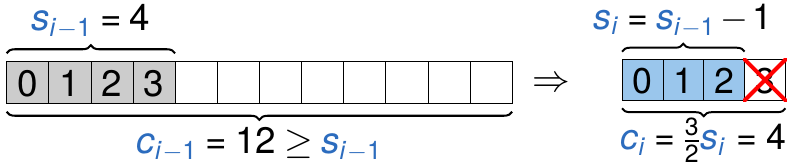
\includegraphics[width=\imgwidth]{array_remove}
      \caption{Remove operation with reallocation}
      \label{fig:remove_array}
    \end{figure}
  \item Amortized runtime:
    \[\sum^n_{k=1}T(O_k)\le 4A\cdot n\]
  \end{itemize}
\end{itemize}

\section{Cache efficiency}
\label{sec:cache_efficiency}
\begin{itemize}
\item Even for the same number of operations, the runtime can differ substantially due to different memory access strategies.
  \begin{itemize}
  \item Example: Adding up array entries in linear order vs. random order.
  \end{itemize}
\item Access times:
  \begin{itemize}
  \item RAM$\rightarrow$Cache: Slow ($\approx 100\mathrm{ns}$)
  \item Cache$\rightarrow$Register: Fast ($\approx 1\mathrm{ns}$)
  \end{itemize}
\item Cache organization:
  \begin{itemize}
  \item The (L1-)cache can hold multiple memory blocks
    ($\approx 100\mathrm{kB}$)
  \item Capacity is reached $\implies$ unused blocks are discarded. Different strategies:
    \begin{itemize}
    \item Least Recently Used (LRU)
    \item Least Frequently Used (LFU)
    \item First in First Out (FIFO)
    \end{itemize}
  \end{itemize}
\item Terminology:
  \begin{itemize}
  \item Memory is divided in blocks of size $B$.
  \item Cache has size $M$ and can store $^M/_B$ blocks.
  \item Data not in cache $\implies$ corresponding block is loaded from memory.
  \end{itemize}
\item Accessing the cache $B$ times:
  \begin{itemize}
  \item Best case: 1 block operation $\rightarrow$ good \emph{locality}
  \item Worst case: $B$ block operations $\rightarrow$ bad \emph{locality}
  \end{itemize}
\item Block loads on cache are called \emph{cache misses}$\rightarrow$ \emph{cache efficiency}
\item Block operations on disk-cache are called \emph{IOs} $\rightarrow$\emph{IO efficiency}
\item Example: Linear order
  \begin{itemize}
  \item Sum up all elements in natural order:
    \[\mathrm{sum(a)}=a[1]+a[2]+...+a[n]\]
  \item Amount of block operations=$\ceil{\frac{n}{B}}$
  \end{itemize}
  
  \begin{figure}[htbp]
    \centering
    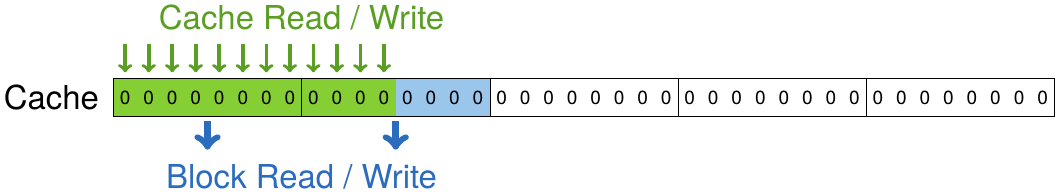
\includegraphics[width=\imgwidth]{good_locality}
    \caption{Good locality of sum operation}
    \label{fig:good_locality}
  \end{figure}
  
\item Example: Random order
  \begin{itemize}
  \item Sum up all elements in random order:
    \[\mathrm{sum(a)}=a[23]+a[42]+...+a[3]\]
  \item Amount of block operations:$n$ in the worst case
  \item Runtime factor difference: $B$
    \begin{figure}[htbp]
      \centering
      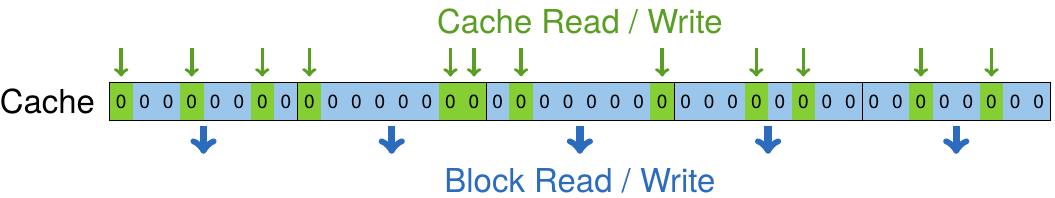
\includegraphics[width=\imgwidth]{bad_locality}
      \caption{Bad locality of sum operation}
      \label{fig:good_locality}
    \end{figure}
  \item Usually, the factor is substantially $< B$ (we might be lucky about the block position)
  \end{itemize}
\end{itemize}

\subsection{Quicksort}
\label{sec:quicksort}
\begin{itemize}
\item Strategy: Divide and conquer
  \begin{itemize}
  \item Task: Divide data into two parts where the left part contains all values $\le$ those in right part
  \item Chose one \emph{pivot}-element
  \item Both parts are sorted reucursively
  \end{itemize}
\item Approach:
  \begin{enumerate}
  \item Pivot in (e.g.) first position, first rearrange list s.t. left part contains small, right part larger elements
    \begin{itemize}
    \item $s$: Start-index of list
    \item $e$: End-index of list
    \end{itemize}
    \begin{figure}[htbp]
      \centering
      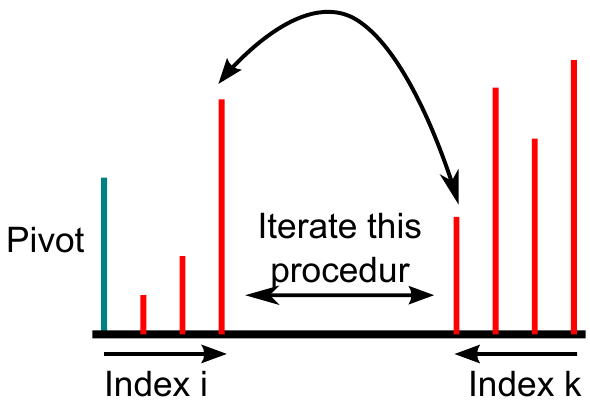
\includegraphics[width=.5\textwidth]{quicksort_schematic}
      \caption{Quicksearch schematic}
      \label{fig:quicksort_schematic}
    \end{figure}
  \item Until $i>k$:
    \begin{itemize}
    \item Increase $i$ until it finds an element $>e_p$
    \item Decrease $k$ until it finds an element $<e_p$
    \item If $i<k$: swap elements $e_i$ and $e_k$
    \end{itemize}
  \item Swap $e_k$ with $e_p$
  \item Call quicksearck on $(s,k-1)$ and $(k+1,e)$
  \end{enumerate}
\item Runtime:
  \begin{itemize}
  \item Best case: $\bigO(n\log n)$
  \item Worst case: $\bigO(n^2)$
  \item Quicksort has quite good locality.
    \begin{figure}[htbp]
      \centering
      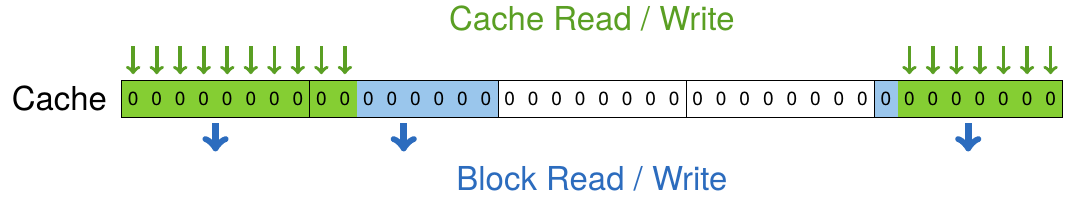
\includegraphics[width=\textwidth]{quicksort_locality}
      \caption{Locality of quicksort}
      \label{fig:quicksort_locality}
    \end{figure}
  \item Block operations: $IO(n):=$ number of block operations for input size $n$
    \begin{align*}
      IO(n)&=\underbrace{A\cdot\frac{n}{B}}_\mathrm{splitting}+\underbrace{2\cdot IO(\frac{n}{2})}_\mathrm{recursive\ sort}\\
           &\le 2A\cdot\frac{n}{B}+4\cdot IO(\frac{n}{4})\\
           &\le 3A\cdot\frac{n}{B}+8\cdot IO(\frac{n}{4})\\
           &\le \dots\\
           &\le kA\cdot\frac{n}{B}+2^k\cdot IO\left(\frac{n}{2^k}\right)\\
           &=\log_2\left(\frac{n}{B}\right)\cdot A\cdot\frac{n}{B}+\frac{n}{B}\cdot IO\left(B\right)\\
           &\le \log_2\left(\frac{n}{B}\right)\cdot A\cdot\frac{n}{B}+A\cdot\frac{n}{B}\\
           &\in \bigO
             \left(
             \frac{n}{B}\cdot\log_2
             \left(
             \frac{n}{B}
             \right)
             \right)
    \end{align*}
  \end{itemize}

\end{itemize}

\subsection{Divide and Conquer}
\label{sec:divide_and_conquer}
\subsubsection*{Concept:}
\begin{itemize}
\item \emph{Divide} the problem into smaller subproblems
\item \emph{Conquer} subproblems through \emph{recursive} solving. If subproblems are small enough, solve them \emph{directly}.
\item \emph{Connect} all solutions of the subproblems to a solution of the full problem.
\end{itemize}

\subsubsection{Features}
\label{sec:O-notation}
\begin{itemize}
\item Requirements:
  \begin{itemize}
  \item Solution of trivial problems needs to be known.
  \item Dividing must be possible.
  \item Sub-Solutions have to be recombinable.
  \end{itemize}
\item Runtime:
  \begin{itemize}
  \item If trivial solution $\in\bigO(1)$
  \item And separation/combination of subproblems $\in\bigO(n)$
  \item And the number of subproblems is finite
  \item[$\implies$] \textbf{Runtime} $\in\bigO(n\cdot\log n)$
  \end{itemize}
\item Suitable for parallel processing, since subproblems are \emph{independent} of each other
\end{itemize}
  
\subsubsection{Implementation}
\label{sec:O-notation}
\begin{itemize}
\item Smaller subproblems are elegant and simple, or it would be better to solve bigger subproblems directly.
\item Recursion depth shouldn't get too big (stack/memory overhead).
\end{itemize}
% TODO: Maybe add the maximum subtotal example?

\subsubsection{Example: Maximum subtotal}
\label{sec:O-notation}
\begin{enumerate}
\item Split sequence in the middle
\item Solve both halves
\item Combine both sub-solutions into a total solution
\item For the case of overlap split, we have to calculate \textrm{rmax} and \textrm{lmax} as well.
\item Solution: $\max(A,B,C)$
  \begin{figure}[htbp]
    \centering
  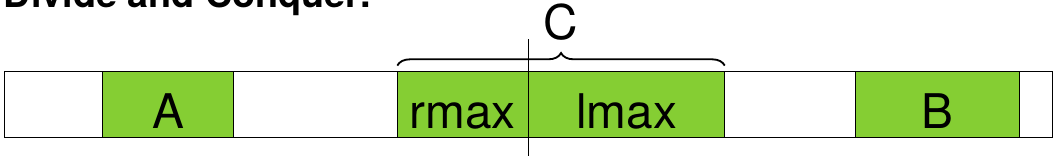
\includegraphics[width=\imgwidth]{maximum_subtotal}
  \caption{Approach to maximum subtotal}
  \label{fig:maximum_subtotal}
\end{figure}
\end{enumerate}

\section{Recursion Equations}
\label{sec:recursion_equations}
\begin{itemize}
\item Recursion equation:
  \begin{equation}
    \label{eq:recursion_equation}
    T(n)=
    \left\{
      \begin{array}{ll}
        f_0(n)&n=n_0\\
        a\cdot T\left(\frac{n}{b}\right)+f(n)&n>n_0
      \end{array}
    \right.
  \end{equation}
  \begin{itemize}
  \item $n=n_0$: Trivial case (usually $\in\bigO(1)$)
  \item $a\cdot T\left(\frac{n}{b}\right)$: Solving of $a$ subproblems with reduced input size $^n/_b$
  \item $f(n)$: slicing and splicing of subsolution
  \item Normally: $a>1$ and $b>1$
  \end{itemize}
\end{itemize}

\subsection{Substitution method}
\label{sec:substitution_method}
\begin{itemize}
\item Guess the solution and prove it with induction
\item Example:
  \begin{equation*}
    T(n)=
    \left\{
      \begin{array}{ll}
        1&n=1 \\
        2\cdot T
        \left(
        \frac{n}{2}
        \right) +n&n>1
      \end{array}
    \right.
  \end{equation*}
\item Assumption: $T(n)=n+n\log_2n$
\item Proof: Induction (base:$n_0=1$, induction step: $n\rightarrow 2n$)
\item Alternative Assumption: $T(n)\in\bigO(n\log n)$
\item Solution: Find $c>0$ with $T(n)\le c\cdot n\log_2n$ (again: induction)
\end{itemize}

\subsection{Recursion tree method}
\label{sec:recursion_tree_method}
\begin{itemize}
\item Can be used to make assumptions about the runtime
\item Example:
  \begin{equation*}
    T(n)=3\cdot T
    \left(
      \frac{n}{4}
    \right)
    +\Theta(n^2)\le 3\cdot T
      \left(
        \frac{n}{4}
      \right)+c\cdot n^2
  \end{equation*}
\begin{figure}[htbp]
  \centering
  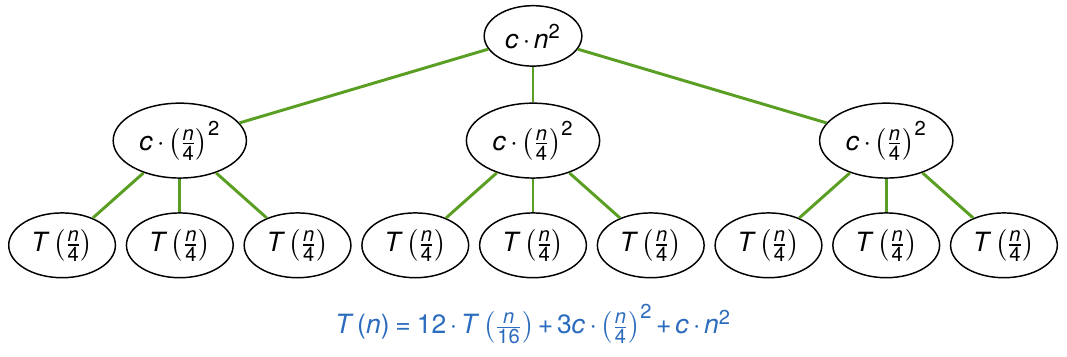
\includegraphics[width=\imgwidth]{recursion_tree_example}
  \caption{Recursion tree of example}
  \label{fig:recursion_tree_example}
\end{figure}
\item Costs of connecting the partial solutions (excludes the last layer):
  \begin{itemize}
  \item Size of partial problems on level $i$: $s_i(n)=
    \left(
      \frac{1}{4}^i\cdot n
    \right)$
  \item Costs of partial problem on level $i$:
    \begin{equation*}
      T_i(n) = c\cdot
      \left(
        \left( \frac{1}{4} \right)^i\cdot n
      \right)^2
    \end{equation*}
  \item Number of partial problems on level $i$: $n_i=3^i$
  \item[$\implies$] Costs on level $i$:
    \begin{equation*}
      T_i(n)=3^i\cdot c\cdot \left( \left( \frac{1}{4} \right)^i\cdot n \right)^2=
      \left( \frac{3}{16} \right)^i\cdot c\cdot n^2
    \end{equation*}
  \end{itemize}
\item Costs of solving the last layer:
  \begin{itemize}
  \item Size of partial problems on the last level: $s_{i+1}(n)=1$
  \item Costs of partial problem on the last level: $T_{i+1}(n)=d$
  \item With this the depth of the tree is:
    \begin{equation*}
      \left( \frac{1}{4} \right)^i\cdot n=1\quad\implies n=4^i\quad\implies i=\log_4 n
    \end{equation*}
  \item Number of partial problems on the last level:
    \begin{equation*}
      n_{i+1}=3^{\log_4 n}=n^{\log_4 3}
    \end{equation*}
  \item[$\implies$] Costs on the last level:
    \begin{equation*}
      T_{i+1}(n)=d\cdot n^{\log_4 3}
    \end{equation*}
  \end{itemize}
\item Total cost:
  \begin{equation*}
    T(n)=\underbrace{\sum^{\log_4(n)-1}_{i=0}\left( \frac{3}{16} \right)^i}_{\mathrm{geometric\ series,\ constant}}\cdot n^2 +
    \underbrace{d\cdot n^{\log_4 3}}_{\log_4 3<1\implies\mathrm{slow\ growth}}\in\bigO(n^2)
  \end{equation*}
\end{itemize}

\subsection{Master theorem}
\label{sec:master_theorem}
\begin{itemize}
\item Appoach to solve for a recursion equation of the form:
  \begin{equation}
    \label{eq:master_theorem_basic}
    \boxed{T(n)=a\cdot T\left( \frac{n}{b} \right)+f(n),\quad a\le 1, b< 1}
  \end{equation}
\item $T(n)$ is the runtime of an algorithm
  \begin{itemize}
  \item ... which divides a problem of size $n$ in $a$ partial problems.
  \item ... which solves each partial problem recursively with a runtime of $T\left( \frac{n}{b} \right)$
  \item ... which takes $f(n)$ steps to merge all partial solutions
  \end{itemize}
\item Three dominations possible:
  \begin{itemize}
  \item Runtime of connecting the solution dominates
  \item Runtime of solving the problems dominates
  \item Both have equal influence
  \end{itemize}
\end{itemize}

\subsubsection{Simple form}
\label{sec:master_simple}
\begin{itemize}
\item Special case with runtime of connecting the solutions: $f(n)\in\bigO(n)$
\item \textbf{Runtime:}
  \begin{equation*}
    T(n)=\left\{
      \begin{array}{lll}
        \Theta\overbrace{(n^{\log_b a})}^{\mathrm{No.\ of\ leaves}}&\mathrm{if\ } a>b & \mathrm{(Branching\ factor\ dominates)}\\
        \Theta(n^{\log_b a})&\mathrm{if\ } a=b& \mathrm{(Balanced\ case)} \\
        \Theta(n)&\mathrm{if\ } a<b& \mathrm{(Shrinking\ factor\ dominates)}

      \end{array}
\right.
  \end{equation*}
\end{itemize}

\subsubsection{General form}
\label{sec:master_general}
\begin{equation}
  \label{eq:master_theorem_general}
  T(n)=a\cdot T\left( \frac{n}{b} \right)+f(n)\quad a\le1,b>1
\end{equation}
\begin{itemize}
\item Case 1: $T(n)\in\Theta(n^{\log_b a})\quad \mathrm{if\ } f(n)\in\bigO(n^{\log_b a-\varepsilon}), \varepsilon>0$\\
  solving the partial problems dominates (last layer, leaves)
\item Case 2: $T(n)\in\Theta(n^{\log_b a}\log n)\quad \mathrm{if\ } f(n)\in\Theta(n^{\log_b a})$\\
  each layer has equal costs, $\log n$ layers
\item Case 3: $T(n)\in\Theta(f(n))\quad \mathrm{if\ }f(n)\in\Omega(n^{\log_b a+\varepsilon}), \varepsilon>0$\\
  Merging the partial solutions dominates.\\
  \textbf{Important:} Regularity condition:
  \begin{equation}
    \label{eq:regularity_condition}
    a\cdot f\left( \frac{n}{b} \right)\le c\cdot f(n),\quad 0\le c\le 1, n>n_0
  \end{equation}
\begin{figure*}[htbp]
  \centering
  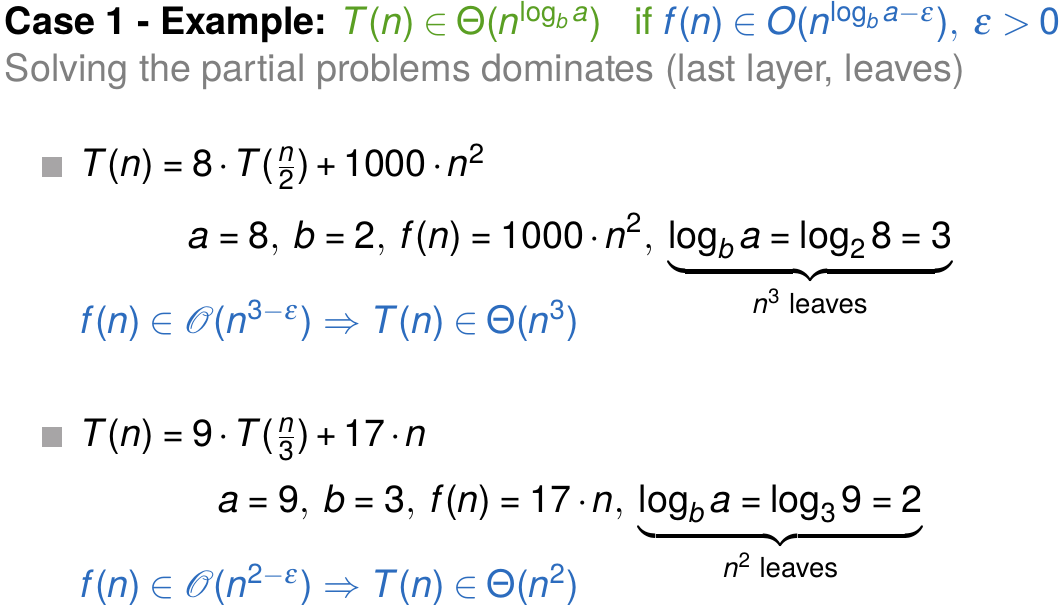
\includegraphics[width=\imgwidth]{master_theorem_ex1}
\end{figure*}
\begin{figure*}[htbp]
  \centering
  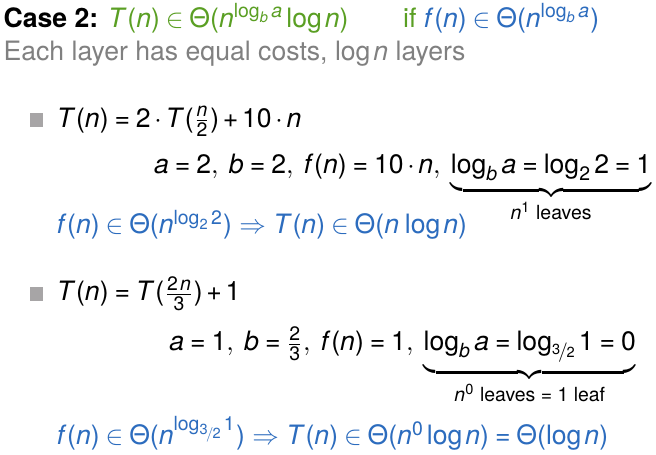
\includegraphics[width=\imgwidth]{master_theorem_ex2}
\end{figure*}
\begin{figure*}[htbp]
  \centering
  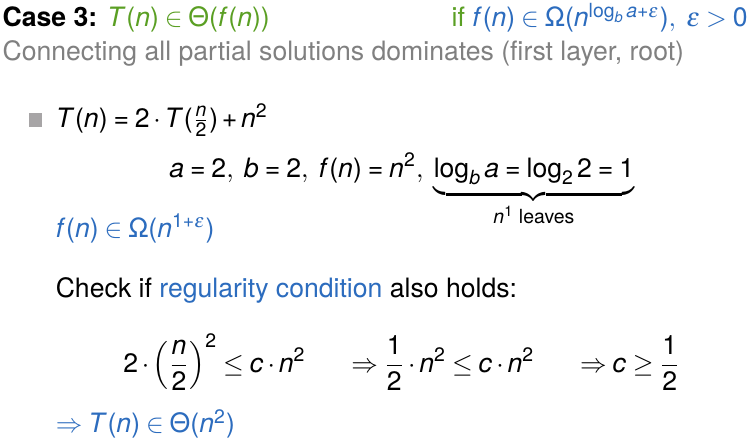
\includegraphics[width=\imgwidth]{master_theorem_ex3}
\end{figure*}
\item The master theorem is not always applicable. Example
  \begin{align*}
    T(n)&=2\cdot T\left( \frac{n}{2}\right) +n\log n \\
    a=2, b&=2, f(n)=n\log n, \underbrace{\log_b a=\log_2 2=1}_{n^1\ \mathrm{leaves}}
  \end{align*}
  \begin{itemize}
  \item $f(n)\notin\bigO(n^{1-\varepsilon})$
  \item $f(n)\notin\Theta(n^1)$
  \item $f(n)\notin\Omega(n^{1+\varepsilon})$
  \item $n\log n$ is \emph{asymptotically} larger than $n$, but not \emph{polynomially} larger.
  \end{itemize}
\end{itemize}

\section{Sorted collections}
\label{sec:sorted_collections}
\begin{itemize}
\item Set of keys, mapped to values
\item Elements are topologically sorted $\le$ by their key
\item The following operations are needed:
  \begin{itemize}
  \item \texttt{insert(key, value)}
  \item \texttt{remove(key)}
  \item \texttt{lookup(key)}: Find the element with the given key, or if not present, return the next bigger one
  \item \texttt{next()}: Returns the element with the next bigger key
  \item \texttt{previous()}: Returns the element with the next smaller key
  \end{itemize}
\end{itemize}

\subsection{Static array}
\begin{itemize}
\item Sorted, static array
\item \texttt{lookup} time: $\bigO(log n)$ \\
  with \emph{binary search}
\item \texttt{next/previous} time: $\Theta(1)$
\item \texttt{insert/remove} time: up to $\Theta(n)$ \\
  We have to copy up to $n$ elements.
\end{itemize}

\subsection{Hash map}
\begin{itemize}
\item \texttt{lookup} time: $\Theta(1)$\\
  if element exists, otherwise result=\texttt{None} 
\item \texttt{next/previous} time: up to $\Theta(n)$ \\
  Order of the elements is independent of the order of the keys.
\item \texttt{insert/remove} time: $\Theta(1)$ \\
  If $m$ is big enough and the hash function is good
\end{itemize}

\subsection{Doubly linked list}
\begin{itemize}
\item \texttt{lookup} time: $\Theta(n)$\\
  Iterate over the elements in the list.
\item \texttt{next/previous} time: $\Theta(1)$\\
  Elements are linked like a chain
\item \texttt{insert/remove} time: $\Theta(1)$
\end{itemize}
\begin{figure}[htbp]
  \centering
  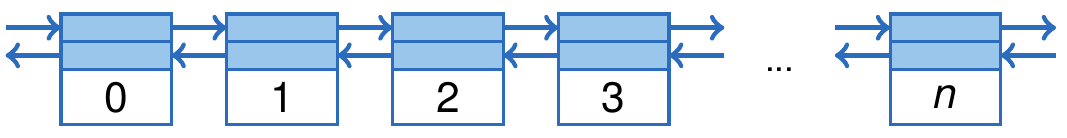
\includegraphics[width=\imgwidth]{doubly_linked_list}
  \caption{Doubly linked list}
  \label{fig:doubly_linked_list}
\end{figure}

\section{Linked lists}
\label{sec:linked_lists}
\begin{itemize}
\item Dynamic datastructure
\item Amount of elements variable
\item Data elements can be simple types upto complex datastructures
\item Elements are linked through references/pointers to the predecessor/successor
\item Singly or doubly linked possible
  \begin{figure}[htbp]
    \centering
    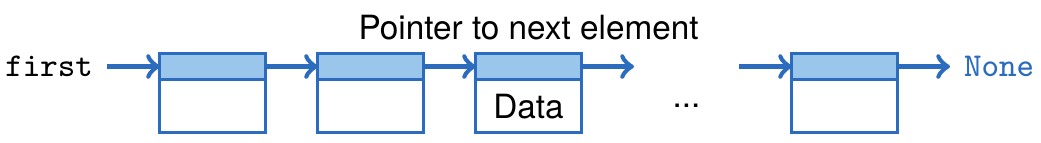
\includegraphics[width=\imgwidth]{singly_linked_list}
    \caption{Singly Linked list}
    \label{fig:singly_linked_list}
  \end{figure}
\item Comparison to an array:
  \begin{itemize}
  \item Needs extra space for storing the pointers
  \item No need for copying elements on \texttt{insert} or \texttt{remove}
  \item The number of elements can be modified without big computational overhead
  \item No direct access of elements (Necessary to iterate over the list)
  \item In general: worse locality than arrays
  \end{itemize}
\end{itemize}

\subsection{List with head/last element pointer}
\begin{itemize}
\item Head element has pointer to first list element
\item Pointer to last element
\item May also hold additional information (e.g.: Number of elements)
\end{itemize}
\begin{figure}[htbp]
  \centering
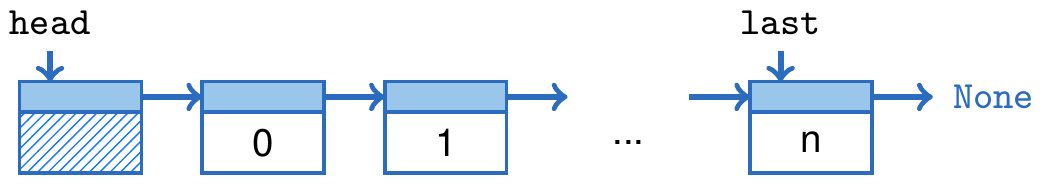
\includegraphics[width=\imgwidth]{header_linked_list}
\caption{Linked list with header}
\label{fig:header_linked_list}
\end{figure}
\subsection{Doubly linked list}
\begin{itemize}
\item Pointer to successor element (last element successor: \texttt{None})
\item Pointer to predecessor element (first element predecessor: \texttt{None})
\item Iterate forward and backward
\end{itemize}
\subsection{Usage}
\begin{itemize}
\item Creating linked lists:
  \begin{itemize}
  \item \texttt{first = Node(7)}
  \item \texttt{first.nextNode = Node(3)}
  \end{itemize}
\item Inserting a node after node \texttt{cur}:
  \begin{enumerate}
  \item \texttt{ins = Node(n)}
  \item \texttt{ins.nextNode = cur.nextNode}
  \item \texttt{cur.nextNode = ins}
  \end{enumerate}% TODO: maybe add graphs? (Lecture 10, p. 29)
\item Removing a node \texttt{cur}:
  \begin{enumerate}
  \item Find predecessor of \texttt{cur} (\texttt{while (pre.nextNode != cur) pre = pre.nextNode;})
    \begin{itemize}
    \item Runtime of $\bigO(n)$
    \item \textbf{Doesn't work on first node!}
    \end{itemize}
  \item \texttt{pre.nextNode = cur.nextNode}
  \item \texttt{delete cur}, or \texttt{cur=None} (automatic if you are a lazy hack who uses garbage collection!)
  \end{enumerate}
\item Removing the first node:
  \begin{enumerate}
  \item \texttt{first = first.nextNode}
  \item \texttt{delete cur}, if no garbage collection
  \end{enumerate}
\item Using a \texttt{head} node:
  \begin{itemize}
  \item Deleting the first node is no special case
  \item Have to consider first node at other operations:
    \begin{itemize}
    \item Iterating all nodes
    \item Counting all nodes
    \item ...
    \end{itemize}
  \end{itemize}
\item \texttt{Head} and \texttt{last} node
  \begin{itemize}
  \item Append elements to the end of the list: $\bigO(1)$
  \item Pointer to \texttt{last} needs to be updated after all operations
  \end{itemize}
  \begin{figure}[htbp]
    \centering
    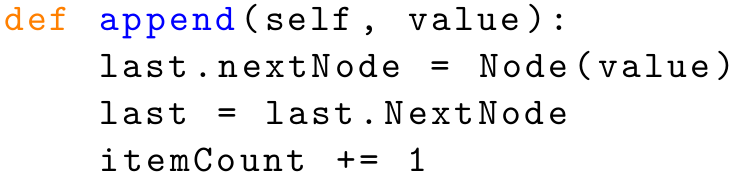
\includegraphics[width=.5\textwidth]{append_linked_algorithm}
    \caption{Algorithm for appending to last element}
  \label{fig:append_algorithm}
\end{figure}
\item \texttt{get(key)}: Iterate the entries until at position ($\bigO(n)$)
\item \texttt{find(value)}: Iterate the entries until value found ($\bigO(n)$)
\end{itemize}

\subsection{Runtime}
\begin{itemize}
\item Singly linked list:
  \begin{itemize}
  \item \texttt{next:} $\bigO{1} $
  \item \texttt{previous:} up to $\Theta(n)$
  \item \texttt{insert:} $\bigO{1}$
  \item \texttt{remove:} up to $\Theta(n)$
  \item \texttt{lookup:} up to $\Theta(n)$
  \end{itemize}
\item Doubly linked list:
  \begin{itemize}
  \item Useful to have a \texttt{head} node.
  \item Only need one \texttt{head} node if we connect the list cyclic (Figure \ref{fig:doubly_linked_list}).
    \begin{figure}[htbp]
      \centering
      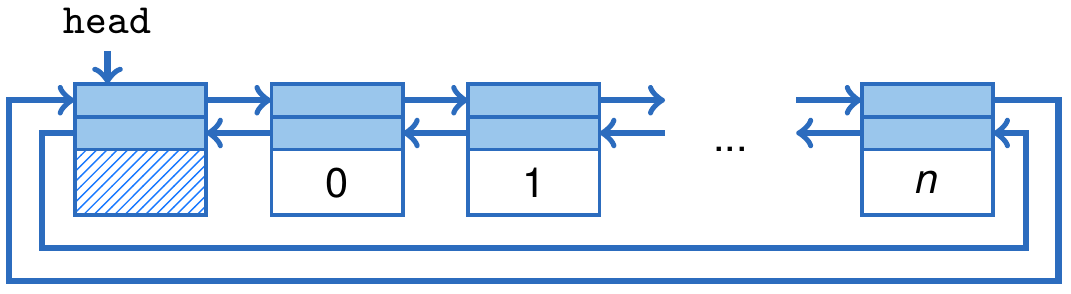
\includegraphics[width=\imgwidth]{cyclic_doubly_linked}
      \caption{Cyclic doubly linked list}
      \label{fig:cyclic_doubly_linked}
    \end{figure}
  \item \texttt{next/previous:} $\bigO(1)$
  \item \texttt{insert/remove:} $\bigO(1)$
  \item \texttt{lookup:} up to $\Theta(n)$ (even if elements are sorted)
  \end{itemize}
\end{itemize}

\section{Binary search tree}
\label{sec:binary_search_tree}
\begin{itemize}
\item \textbf{Principle}:
  \begin{itemize}
  \item Define a total order (e.g. $\le$, $\ge$)
  \item All nodes of the left subtree have \emph{smaller keys} than the current node.
  \item All nodes of the right subtree have \emph{bigger keys} than the current node.
  \item The next highest element of the current node is the leftmost element from the left subtree.
  \item The next lowest element of the current node is the rightmost element from the right subtree.
  \end{itemize}
  \begin{figure}[htbp]
    \centering
    \begin{subfigure}[b]{.4\textwidth}
      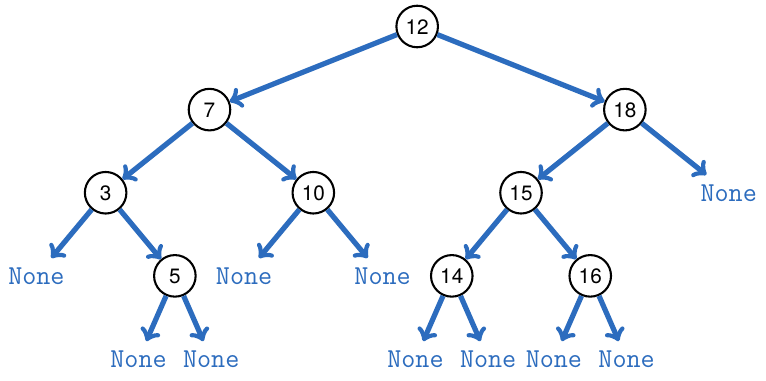
\includegraphics[width=\textwidth]{search_tree_ref}
      \caption{Binary search tree with references}
      \label{fig:binary_search_tree}
    \end{subfigure}
    ~
    \begin{subfigure}[b]{.47\textwidth}
      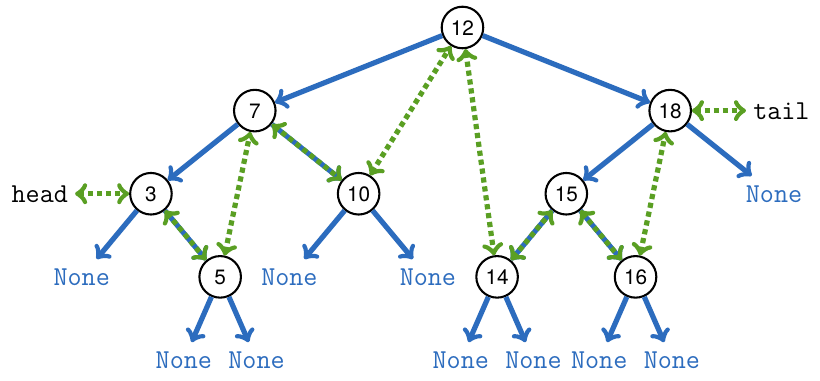
\includegraphics[width=\textwidth]{search_tree_linked}
      \caption{Binary search tree with doubly linked list}
    \end{subfigure}
  \end{figure}
\item \textbf{Runtime:}
  \begin{itemize}
  \item \texttt{next/previous}: $\bigO(1)$
  \item \texttt{insert/remove}: $\bigO(\log n)$
  \item \texttt{lookup:} up to $\Theta(n)$
  \end{itemize}
\item \textbf{Implementation}:
  \begin{itemize}
  \item We link all nodes through pointers/references
  \item Each node has a pointer/reference to its' children (\texttt{leftChild/rightChild})
  \end{itemize}
\item Implementation on steroids (with links):
  \begin{itemize}
  \item Sorted doubly linked list of all elements
  \item[$\implies$] Efficient implementation of \texttt{next/previous}
  \end{itemize}
\item \texttt{Lookup(key)}: ``Search element. If not found, return element with next (bigger) key''
  \begin{itemize}
  \item Start at root
  \item Go down left/right recursively until found, or \texttt{None}
  \item If \texttt{None}: return next biggest element
  \end{itemize}
\item \texttt{Insert(key, value)}:
  \begin{itemize}
  \item Search for key in tree
  \item If found: $\rightarrow$ replace value with the new one
  \item Else: insert new node at the corresponding \texttt{None} entry
  \end{itemize}
\item \texttt{Remove(key)}: (quite tricky)
  \begin{enumerate}
  \item Node has no \texttt{children}:
    \begin{itemize}
    \item Find \texttt{parent} of the node.
    \item Set the left/right \texttt{child} of the \texttt{parent} node to \texttt{None}.
    \end{itemize}
  \item Node has one \texttt{child}:
    \begin{itemize}
    \item Find the \texttt{child} of the node.
    \item Find the \texttt{parent} of the node.
    \item set the left/right \texttt{child} of the \texttt{parent} node to the node's \texttt{child}.
    \end{itemize}
  \item Node has two children
    \begin{itemize}
    \item Find the nodes' \texttt{successor}.
    \item Replace the node with its' \texttt{successor}
    \item Delete the \texttt{successor}
    \end{itemize}
\end{enumerate}
\item Runtime of \texttt{insert()} and \texttt{lookup()}:
  \begin{itemize}
  \item Up to $\Theta(d)$ ($d:=$ depth of the tree)
  \item Best case $d=\log n$: $\Theta(\log n)$
  \item Worst case $d=n$: $\Theta(n)$ (tree degenerated)
  \item For consistent runtime of $\Theta(\log n)$, we have to \emph{rebalance} the tree.
  \end{itemize}
  \begin{figure}[htbp]
    \centering
    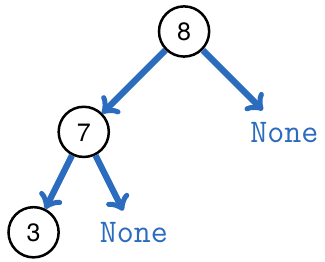
\includegraphics[height=20mm]{search_tree_degenerated}
    \caption{Degenerated search tree}
  \end{figure}
\end{itemize}

\section{Balanced search trees}
\label{sec:balanced_search_trees}
\begin{itemize}
\item How do we fix degenerated trees? $\rightarrow$ rebalancing!
\item Rebalancing possibilities:
  \begin{itemize}
  \item AVL-Tree:
    \begin{itemize}
    \item Binary tree with 2 children per node
    \item Balancing via ``rotation''
    \end{itemize}
  \item (a,b)-Tree, or B-Tree:
    \begin{itemize}
    \item Nodes have between $a$ and $b$ children
    \item Balancing through \emph{splitting} and \emph{merging} nodes.
    \item Used in data bases and file systems
    \end{itemize}
  \item Red-Black-Tree:
    \begin{itemize}
    \item Binary tree with black and red nodes
    \item Balancing through \emph{rotation} and \emph{recoloring}
    \item Can be interpreted as (2,4)-tree
    \end{itemize}
  \end{itemize}
\end{itemize}
\subsection{AVL-Tree}
\label{sec:avl-tree}
\begin{itemize}
\item \textbf{A}delson-\textbf{V}elskii, \textbf{L}andis (1963)
\item Search tree with modified \texttt{insert()} and \texttt{remove} operations, while satisfying a \emph{depth condition}.
\item Prevents degeneration
\item \textbf{Depth condition:} Highest possible height difference of left and right subtree = 1
\item[$\implies$] Depth of tree is always $\bigO(\log n)$
\begin{figure}[htbp]
  \centering
  \begin{subfigure}[b]{.3\textwidth}
    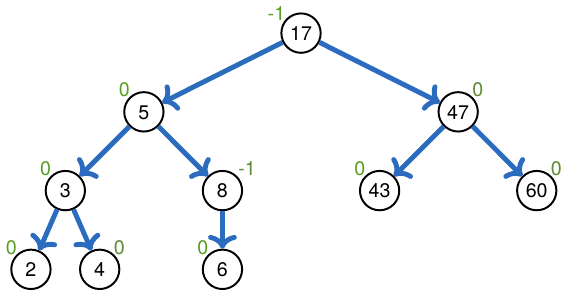
\includegraphics[width=\textwidth]{avl_tree}
    \caption{AVL tree}
  \end{subfigure}
  \begin{subfigure}[b]{0.25\textwidth}
    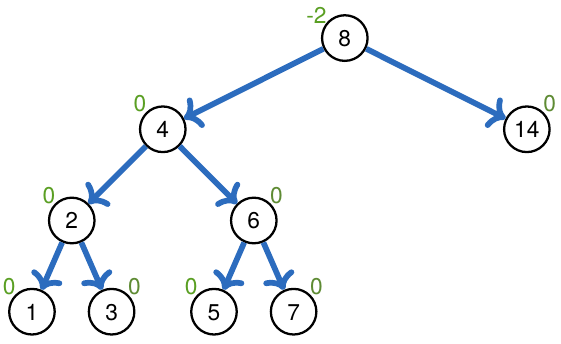
\includegraphics[width=\textwidth]{avl_tree_bad}
    \caption{Not an AVL tree}
  \end{subfigure}
\end{figure}\newpage
\item \textbf{Rotation:}
  \begin{figure}[!htbp]
    \centering
    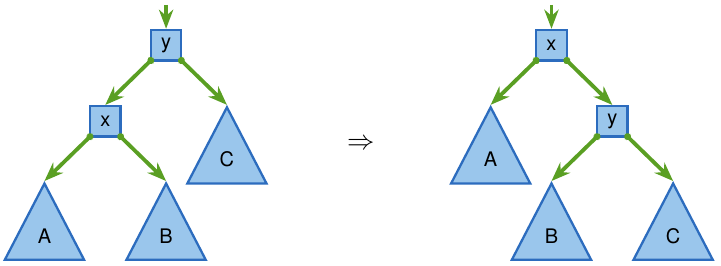
\includegraphics[width=\imgwidth]{rotation}
    \caption{Rotation principle}
    \label{fig:rotation}
  \end{figure}

  \begin{itemize}
  \item \texttt{Parent-Child} relations are swapped for nodes which violate the depth-condition.
  \item Attention: in this example, $x$'s smaller subtree becomes $y$'s larger subtree!
  \end{itemize}
\item If a height difference of $\pm2$ occurs after an \texttt{insert/remove}, the tree is rebalanced.
\item \textbf{Disadvantages:}
  \begin{itemize}
  \item Update cost is no longer an amortized $\bigO(1)$!
  \item More memory consumption for depth values
  \end{itemize}
\item[$\implies$] Better option: (a,b)-Trees, a.k.a. b-trees (b for ``balanced'')
\end{itemize}
\subsection{(a,b)-tree}
\label{sec:ab-tree}
\begin{itemize}
\item \textbf{Principle}:
  \begin{itemize}
  \item Save a varying number of elements per node
  \item All leaves have the same depth
  \item Each inner node has $\ge a$ and $\le b$ nodes (exeption: root node)
  \item Subtrees are located ``between'' the elements.
  \item $a\ge 2, b\ge 2a-1$
  \end{itemize}
  \begin{figure}[htbp]
    \centering
    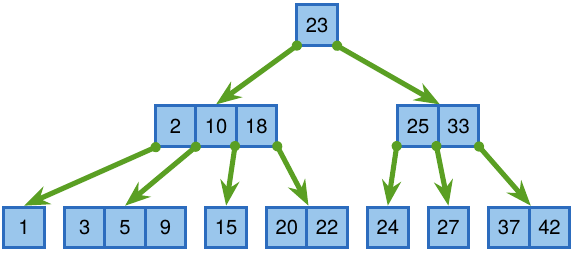
\includegraphics[width=0.5\textwidth]{2-4_tree}
    \caption{Example of an (2,4)-tree}
    \label{fig:2-4_tree}
  \end{figure}
\item \texttt{lookup}: Same as in binary search tree
\item \texttt{insert}:
  \begin{itemize}
  \item Search the position to insert (always a leaf).
  \item Insert node
  \item Check if maximum number of nodes are exceeded.
  \item If yes: Split the node!
  \item[$\implies$] Two new nodes with $\ceil{\frac{b-1}{2}}$ and $\floor{\frac{b-1}{2}}$ elements.
  \item Checking the maximum number of nodes cascades up.
  \item If we have to split the root node, we create a new one afterwards.
  \end{itemize}
  \begin{figure}[htbp]
    \centering
    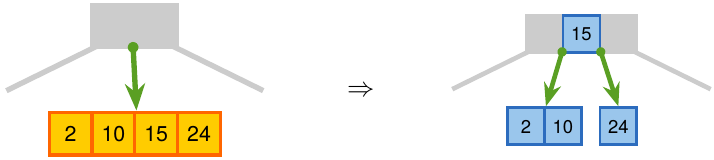
\includegraphics[width=\imgwidth]{split_node}
    \caption{Splitting a node}
    \label{fig:split_node}
  \end{figure}
\item \texttt{remove}:
  \begin{itemize}
  \item Search the element ($\bigO(\log n)$)
  \item Case 1: Element is contained by a leaf $\implies$ remove it!
  \item Case 2: Contained by an inner node
    \begin{itemize}
    \item Search the \textbf{successor} in the \textbf{right} subtree. (leftmost element of rightmost subtree, always contained by a leaf)
    \item Replace the element with its' successor and delete the successor from the leaf
    \end{itemize}
    \item \textbf{Attention:} If size of leaf $< a$!
    \item[$\implies$] \textbf{Rebalance} the tree:
      \begin{itemize}
      \item Case 1: If the left or right neighbour node has leafs to spare, \textbf{get that one}
        \begin{figure}[htbp]
          \centering
          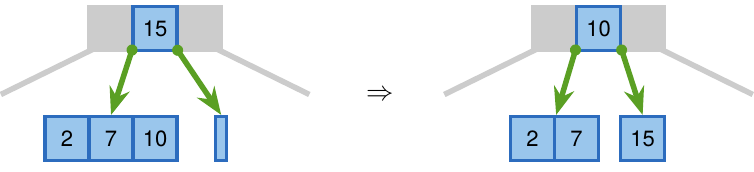
\includegraphics[width=\imgwidth]{borrowing_element}
          \caption{borrowing an element}
          \label{fig:borrowing_element}
        \end{figure}
      \item Case 2: \textbf{Combine} the node with its' neighbour\\
        \begin{figure}[htbp]
          \centering
          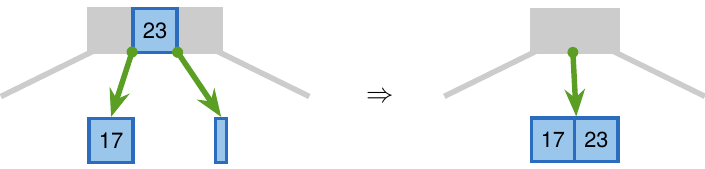
\includegraphics[width=\imgwidth]{combine_neighbour}
          \caption{Combining with neighbour}
          \label{fig:combine_neighbour}
        \end{figure}
        \textbf{Check if we have to cascade upwards!}
      \item If the root has only one child left, that child can become root.
      \end{itemize}
    \end{itemize}
  \end{itemize}
  
\subsubsection*{Runtime of \texttt{lookup, insert} and \texttt{remove}}
\begin{itemize}
\item All operations: $\bigO(d), d:=$depth of the tree
\item Each node (except root) has more than $a$ children\\
  $\implies n\ge a^{d-1}$ and $d\le 1+\log_a n \in \bigO(\log_a n)$
\item \texttt{lookup}: $\in\Theta(d)$
\item \texttt{insert/remove}: often only in $\bigO(1)$
\item Only in worst case, we have to split or combine all nodes cascading up to root
\end{itemize}

\subsubsection{Analysis of $b\ge2a$}
\begin{itemize}
\item nodes with \textbf{2, or 4 children} are expensive for delete and add respectively (borrowing, or splitting, possibly cascading up).
\item[$\implies$] \textbf{3 children} are harmless:
  \begin{itemize}
  \item $\Phi_i$:= Potential of the tree after the $i$-th operation.
  \item[=] the amount of harmless nodes (size 3)
  \item After expensive operation the tree is in a stable state. %TODO: Include proof? Lecture 11
  \item Takes some time until the next expensive operation occurs.
  \item Same principle of dynamic arrays: \textbf{Overallocate} clever, to get an amortized runtime of $\bigO(1)$
  \end{itemize}
\end{itemize}

\subsection{Red-Back-Tree}
\begin{itemize}
\item Binary tree with \textrm{red} and \textrm{black} nodes
\item Number of black nodes on path to leaves is equal
\item Can be interpreted as (2,4)-tree
\end{itemize}
\begin{figure}[htbp]
  \centering
  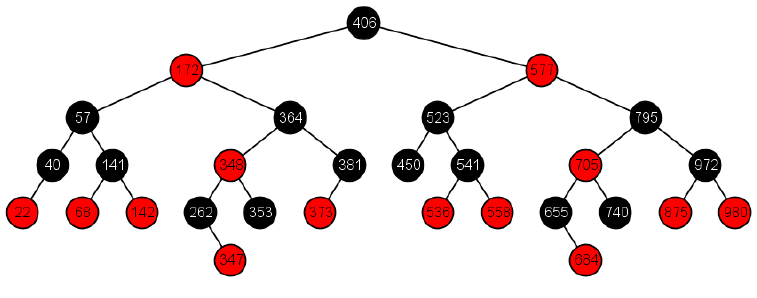
\includegraphics[width=\imgwidth]{red-black_tree}
  \caption{Example of a red-black-tree}
  \label{fig:red-black_tree}
\end{figure}

\end{document}

%%% Local Variables:
%%% mode: latex
%%% TeX-master: t
%%% End:
 